%!TEX program = xelatex
% 完整编译: xelatex -> bibtex -> xelatex -> xelatex

\documentclass[lang=cn,11pt,a4paper,cite=authoryear]{elegantpaper}
\usepackage{indentfirst}
\setlength{\parindent}{2em}

\title{编译原理实验三:中间代码生成}
\author{林搏海 1190202128}
\institute{{哈尔滨工业大学} {物联网工程}}
\date{\zhtoday}


% 本文档命令
\usepackage{array}
\newcommand{\ccr}[1]{\makecell{{\color{#1}\rule{1cm}{1cm}}}}

\begin{document}

\maketitle

\begin{abstract}
\hspace*{0.7cm}在Lab1中,我们实现了基于Flex的词法分析和基于Bison的语法分析,在Lab2中,我们实现了语法制导的语义翻译过程,构建了语法分析树,并且进行了相应的语义检查。本次实验在前两次实验的基础之上进行了中间代码翻译,将源代码翻译为中间代码的过程是在之前构建的语法分析树上递归进行的,此外,中间代码的存储采用了链表的结构进行顺序存储,该方式实现简单,并且在其中进行查询和删改的操作都较为高效。
\keywords{语法分析树, 中间代码, 链表}
\end{abstract}



\section{中间代码生成}
\subsection{代码生成过程概述}
我们通过遍历实验一中的语法分析树来进行中间代码生成,中间代码生成主要是为源程序生成相应的中间表示形式,这样的表示形式独立于源代码和目标代码,从而起到了前后端分离的作用。与实验二相同的是,中间代码的生成也是进入 ExtDefList 后的事,因此我们只需要遍历语法树,根据实验指导书为我们提供的翻译规则进行中间代码的生成即可。生成的中间代码我们将其加入中间代码存储链表中。另外,我们对中间代码的生成没有做太多优化,主要对直接使用的符号和立即数进行了一步去掉一步创建新临时变量的优化,所以在最后生成的代码中可能会出现一些临时变量和label的冗余。

\subsection{中间代码链表原理及其实现}
在遍历语法分析树进行中间代码翻译的时候,我们需要找到ExtDefList出现的位置,然后再递归的进行翻译,递归的翻译代码的过程通过递归调用函数genInterCodes函数实现。genInterCodes函数则是调用了translateExtDefList模块进行中间代码翻译。translate系列函数是我们为教材不同的中间代码翻译规则编写的翻译函数模块,帮助实现自顶向下的递归中间代码生成。在translate系列函数的最底层,执行的是genInterCode函数,该函数为了适应不同类型中间变量的翻译要求,采用了变长参数的设计,使得函数本身简单易懂,复用性也得到了很大的提升。同时,函数内部通过switch分支语句控制不同类型的中间代码翻译,使得代码简介高效。最终,genInterCode函数生成的中间代码我们通过addInterCode加入到中间代码链表中,中间代码链表的声明如图\ref{pic1}所示:\par


对于中间代码表的初始化部分如图\ref{pic2}所示。\par

\begin{figure}[htbp]
	\centering
	\begin{minipage}[t]{0.48\textwidth}
		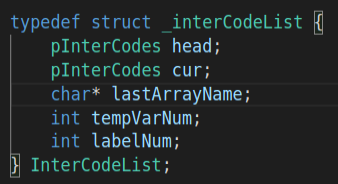
\includegraphics[width=2.3in]{pics//p1.png}
		\caption{中间代码链表定义}
		\label{pic1}
	\end{minipage}
	\begin{minipage}[t]{0.48\textwidth}
		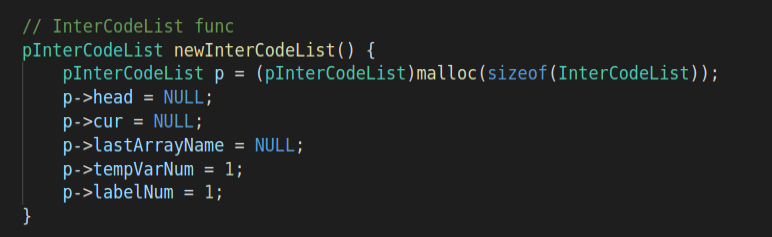
\includegraphics[width=4.0in]{pics//p2.png}
		\caption{中间代码链表初始化}
		\label{pic2}
	\end{minipage}
\end{figure}


此外,为了进行空间管理,防止出现内存泄漏的情况,我们对于中间代码链表空间进行了严格的释放流程,当有需要的时候,我们会删除中间代码并且释放相应的空间,如图\ref{pic3}:\par
\begin{figure}[h]
	\centering
	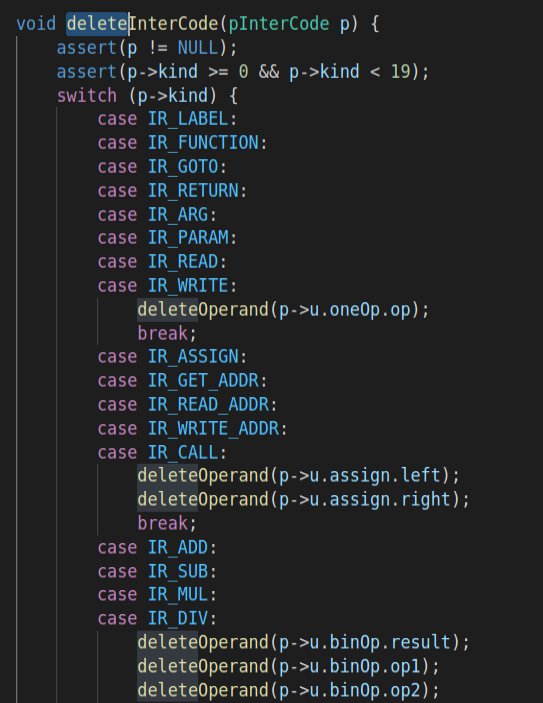
\includegraphics[width=4.2in]{pics//p3.png}
	\caption{中间代码空间释放}
	\label{pic3}
\end{figure}



\section{主程序模块}
为了方便编译和调试,我们将main函数放在了main.c文件中,其具体逻辑入下:首先,读入cmm文件,调用yyparse()函数对其进行词法分析和语法分析,并且建立相应的语法分析树。如果词法分析阶段或者是语法分析阶段检测到错误,那么我们就调用我们自己重写的error函数进行报错;如果此过程没有错误,那么我们就初始化符号表,并且从根节点开始遍历整个语法分析树,并且执行对应的分析语句,如果出现语义错误,则输出相应的错误类型。如果整个程序没有任何的词法语法或者是语义错误,那么,我们就生成中间代码链表,并且再次遍历语法分析树,从而进行中间代码翻译,在结束中间代码翻译之后,如果没有出现语法错误,那么就将中间代码ir文件输出到我们指定的目录下。
\section{编译执行方式}
程序的正确编译执行需要以下10个文件:inter.h,inter.c,enum.h, node.h, lexical.l, main.c, syntax.y, makefile, semantic.h, semantic.c, 只需要确保他们处在同一个目录下,然后执行make命令调用makefile文件执行自动编译即可。使用make命令将得到可执行文件parser,我们需要对于每一个测试文件手动输入测试用例,并且得到对应的.ir格式中间文件,将其输出到output文件夹中(test1.cmm和test2.cmm对应的中间代码文件out1.ir和out2.ir已在output文件夹中),执行parser的命令格式为(在src目录下):./parser ../test/test1.cmm ../output/out1.ir。对于得到的ir文件,我们只需要将其放入irsim虚拟机中执行即可验证其正确性,如图\ref{pic4}

\begin{figure}[h]
	\centering
	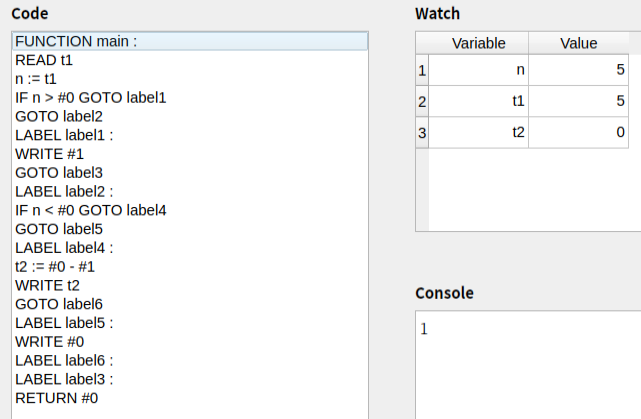
\includegraphics[width=4.5in]{pics//p4.png}
	\caption{irsim执行中间代码结果}
	\label{pic4}
\end{figure}

\end{document}
